% Lists frame
\section{GPC}
\begin{frame}{Wielowymiarowy GPC}
Schemat projektowania wielowymiarwego algorytmu GPC:
\begin{itemize}
    \item Wyznaczenie wielowymiarowej odpowiedzi impulsowej
    \item Wyznaczenie modelu obiktu w postaci dyskretnego równania różnicowego
    \item Wyznaczenie predyktora minimalnowariancyjnego
    \item Wyznaczenie składowej wymuszanej i swobodnej predykcji wyjść
    \item Wyznaczenie odpowiedzi swobodnej
    \item Wyznaczenie wektora optymalnych przyrostów sterowań
\end{itemize}
Wszystkie sygnały sterujące wpływają na sygnały wyjściowe. 
\end{frame}


\begin{frame}{Wielowymiarowy GPC}
Wyznaczenie wielowymiarowej odpowiedzi impulsowej:
	\begin{center}
		\begin{figure}[H]
            		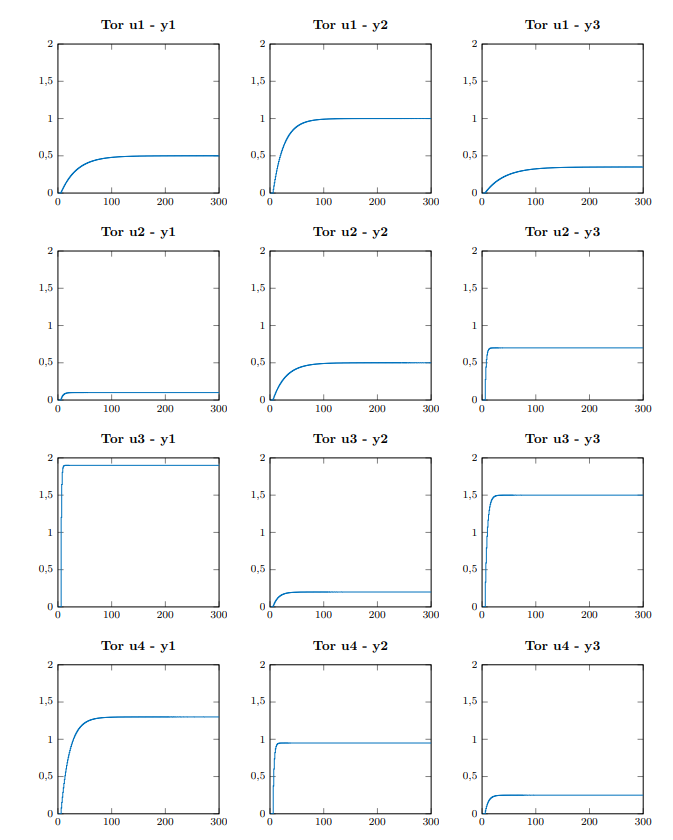
\includegraphics[scale=0.25]{images/PIDtory.png}
          			 \caption{Wielowymiarowa odpowiedź impulsowa}
		\end{figure}
	\end{center}
\end{frame}

\begin{frame}{Wielowymiarowy GPC}
Określenie pętli regulacji:
	\begin{center}
		\begin{figure}[H]
            		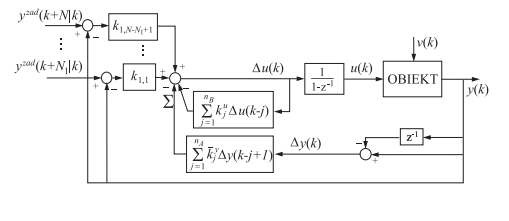
\includegraphics[scale=0.7]{images/SISOGPC.png}
          			 \caption{Schemat układu regulacji}
		\end{figure}
	\end{center}
\end{frame}

\begin{frame}{Wielowymiarowy GPC}
Wyniki działania:
	\begin{center}
		\begin{figure}[H]
            		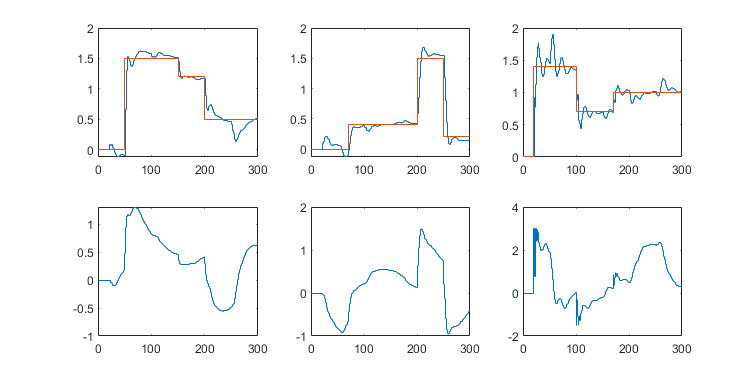
\includegraphics[scale=0.5]{images/PID_wyniki.png} %%do poprawy jak już będą ładne
          			 \caption{Wyniki regulacji}
		\end{figure}
	\end{center}
\end{frame}
